\documentclass[10pt,a4paper]{report}

\usepackage[utf8]{inputenc}
\usepackage{amsmath}
\usepackage{amsfonts}
\usepackage{amssymb}
\usepackage{graphicx}
\usepackage{hyperref}
\usepackage[left=2cm,right=2cm,top=2cm,bottom=2cm]{geometry}

\title{Product Vision and Planning}
\author{Programming Life group 2\\
	\begin{tabular}{c c c}
	\hline 
		Derk-Jan Karrenbeld & 4021967 & 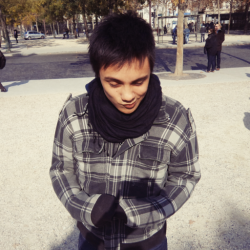
\includegraphics[scale=0.2]{../img/DJ.png}\\ 
		Joost Verdoorn & 1545396 & 
\includegraphics[scale=0.2]{../img/Yoloost.png}\\ 
		Steffan Sluis & 4088816 & 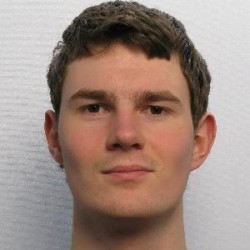
\includegraphics[scale=0.2]{../img/SS.jpeg}\\ 
		Tung Phan & 4004868 & 
\includegraphics[scale=0.2]{../img/TP.jpeg}\\ 
		Vincent Robbemond & 4174097 & 
\includegraphics[scale=0.2]{../img/VR.jpeg}\\ 
		\hline 
	\end{tabular} 
}
\date{\today}

\begin{document}
	\maketitle

	\section*{Preface}
		This document is a draft for the product vision and planning for the Context Project `Programming Life: Synthetic Biology'. It’s a proposition for the project structure, workflow and product target result that we will engage in and with during the period of the course. It contains a schedule with set dates, milestones and goals to be achieved and is a guideline for the work that should be done. The contents of this document are subject to changes and should be regarded as such.

	\setcounter{section}{0}
	\setcounter{secnumdepth}{3}
	\setcounter{tocdepth}{5}
	\renewcommand*\thesection{\arabic{section}}
	
	\pdfbookmark{\contentsname}{toc}
	\tableofcontents

	\clearpage

	\section{Introduction}
		Synthetic biologists try to create cells that serve a specific purpose, for instance the creation of a product from a source metabolite while maintaining a predetermined rate of cell growth. Before they accomplish this, they would like to simulate the internal workings of cells by simulating their mutual influence on one another using combinations of several differential equations which influence each other. 
By varying the properties, i.e. the factors and values used by these equations, the biologists can simulate the interplay of elements within the cell based on that set of properties. 
However, the complexity of the simulation can be daunting as well as time consuming if done on paper or programmed by hand per set of factors.\\

GigaBase is an intuitive application that should overcome these problems by providing a GUI and allowing the simulation of an extensive number of modules. It allows the user to specify properties of the cell and the elements within, such as the flow rate of a transporter or the initial amount of substrate outside of the cell. This way, a cell can be modelled by solving a system of ODEs representing the specified properties and interactions of each of its modules. By using this application, the user can efficiently find the optimal properties with less work to get the desired outcome, such as maximizing the product of a cell. The user also does ot have to worry about performing calculations which are prone to error and take a long time to perform.
\\

This product will be developed using the Scrum methodologies and the development wil be iterated in weekly sprints.

	\clearpage

	\section{Product}
		This section holds the main product vision, the high level product backlog and a general roadmap for the contents of the product during the project.
		\subsection{Product Vision}

			\textbf{FOR} Synthetic Biologists \textbf{WHO LIKE TO} create cells that work in certain ways, GigaBase \textbf{IS AN} application \textbf{THAT} allows the user to simulate a cell's interactions with itself and its environment by selecting modules that make up the cell, varying their properties and the environment, simulating the interplay of elements in the cell and visualising the outcome of the interactions in a graph. \textbf{UNLIKE} modelling the cell by generating and solving an ODE \textbf{OUR SERVICE} fast-tracks designing a cell by providing a GUI, enforces constraints for the entered values of the ODEs to minimize errors, saves time by reusing previous designs and solves the ODE, taking out a possibility for human error.

		\subsection{High-level product backlog}
			\textbf{A user can model a cell by selecting modules.}\\
			\indent
				\textit{Note: A GUI provides the modules needed to model a cell.}\\
			\textbf{A user can see the output of a model when it is simulated over a period of time.}\\
			\indent
				\textit{Glossary: A model is a selection of modules with their properties and initial conditions set.}\\
			\indent
				\textit{Note: At least one graph per module shows the output. The graph shows the concentrations of the substances modeled by the module such as DNA and proteins. The simulation period can be changed.}\\
			\textbf{A user can set the properties of modules and cell environment.}\\
			\indent
				\textit{Note: A GUI lists the properties and allows changing.}\\
			\textbf{A user can export the results of the design to a report.}\\
			\indent
				\textit{Note: output file(s) such as HTML, Excel, SBML and/or PDF.}\\
			\textbf{A user can save and load models}.\\
			\indent
				\textit{Note: Models are serializable. A database is used for storage.}\\
			\textbf{A user gets feedback on his model.}\\
			\indent
				\textit{Note: Visual feedback such as constraints for modules, errors and possible optimizations.}\\
			\textbf{A user can add or change modules.}\\
			\indent
				\textit{Note: The differential equation(s) of a module should be changeable. The inter-module constraints should be changed accordingly.}\\
			\textbf{A user can undo an action.}\\
			\indent
				\textit{Note: Actions such as adding/editing/removing modules.}\\
			
		\clearpage
		\subsection{Roadmap}
			\begin{figure}[htb]
			\centerline{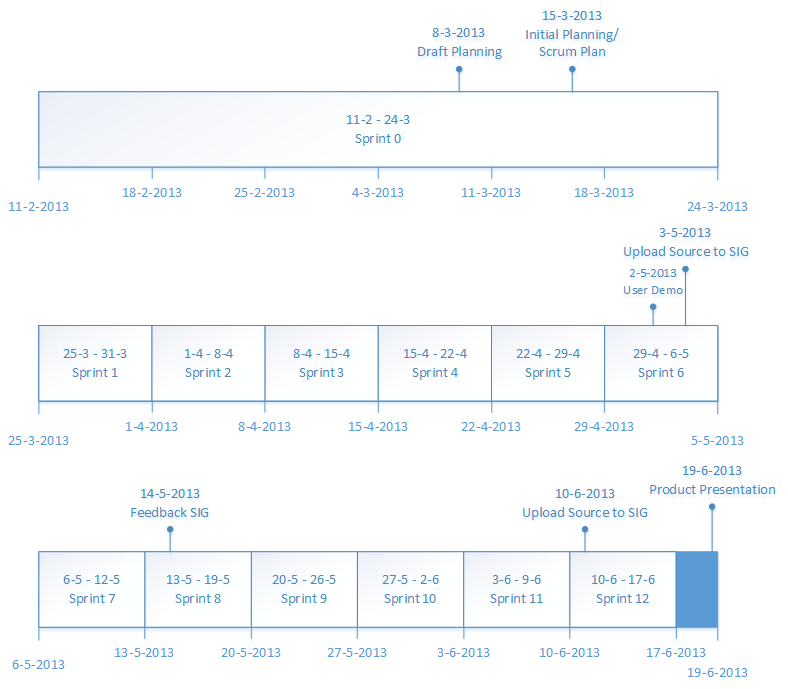
\includegraphics[scale=0.8]{Roadmap.png}}
			\caption{Roadmap}
			\label{fig: Roadmap}
			\end{figure}	
			\subsubsection*{Sprint 0}
				\textbf{Q3/W4 Draft planning:}\\ The product and domain are researched, the product vision and high-level product backlog are devised with initial listing of user stories composed. The user stories can be found under the product backlog section.\\
				\textbf{Q3/W5 Initial planning:}\\ The user story list is fine-tuned and tasks are devised for the first sprints.\\
				The user stories can be found under the product backlog section. After this sprint all code for internal workings should be present.\\		
				\textbf{Q3/W6}\\
				Toolchain needed to develop the code is set up. Basic module and cell classes are made and properly tested.
			\subsubsection*{Sprint 1 (Q3/W7)}
				A cell can be created by selecting modules from a list. Start working on integration tests.
			\subsubsection*{Sprint 2 (Q3/W10) Demo product}
				A basic visualisation of the internal workings is present. This consists of at least one graph per module that indicates the concentration over time. A set of modules with predefined property values is available for cell modelling. Equations are solved using an ODE solver.
			\subsubsection*{Sprint 3 (Q4/W1)}
				Initial rigorous acceptance tests, as the next sprint requires a product demo. Substrates can now be added to the cell. Tests are run automatically using Continuous Integration. Release first version with basic functionality.
			\subsubsection*{Sprint 4 (Q4/W2)}
				All events should now be handled by an Event Manager. There should be a reasonable amount of tests covering a reasonable amount of code, i.e. around 80\%. Release the demo version for the product demo.
			\subsubsection*{Sprint 5 (Q4/W3)}
				The GUI now provides a graphical way to add modules to the cell it also provides a way to control the simulation of the cell. The cell models created can now be saved and loaded. An API is also provided. Preparation for SIG evaluation by cleaning up redundant code and adding documentation where needed.
			\subsubsection*{Sprint 6 (Q4/W4)}
				HTML/PDF/EXCEL reports can now be generated from created cell models, containing parameter values and graphs from simulations. A user can now change module constants. Connections between modules are visualised. 
			\subsubsection*{Sprint 7 (Q4/W5)}
				Bug-fixes, acceptance tests and final review of code. Implement improvements based on SIG feedback. A user can use the undo function in the GUI. Feedback on module constraints and errors is visible.
			\subsubsection*{Sprint 8 (Q4/W6)}
				Code cleanup, maintenance, bug fixing and other possible improvent to the system.
			\subsubsection*{Sprint 9 (Q4/W7)}
				Feedback on optimisation is now visible in the application. 
			\subsubsection*{Sprint 10 (Q4/W8) Final product}
				All remaining bugs are fixed. All tests should pass with a good coverage, i.e. around 80\%. Prepare for product presentation. Release presentation demo version.

	\clearpage

	\subsection{Product mockup}
		In the image below is the mockup we drew of the product graphical user interface, showing a cell and its modules. The modules which interact with each other are connected and clicking on the modules reveals more information.
		\begin{figure}[htb]
			\centerline{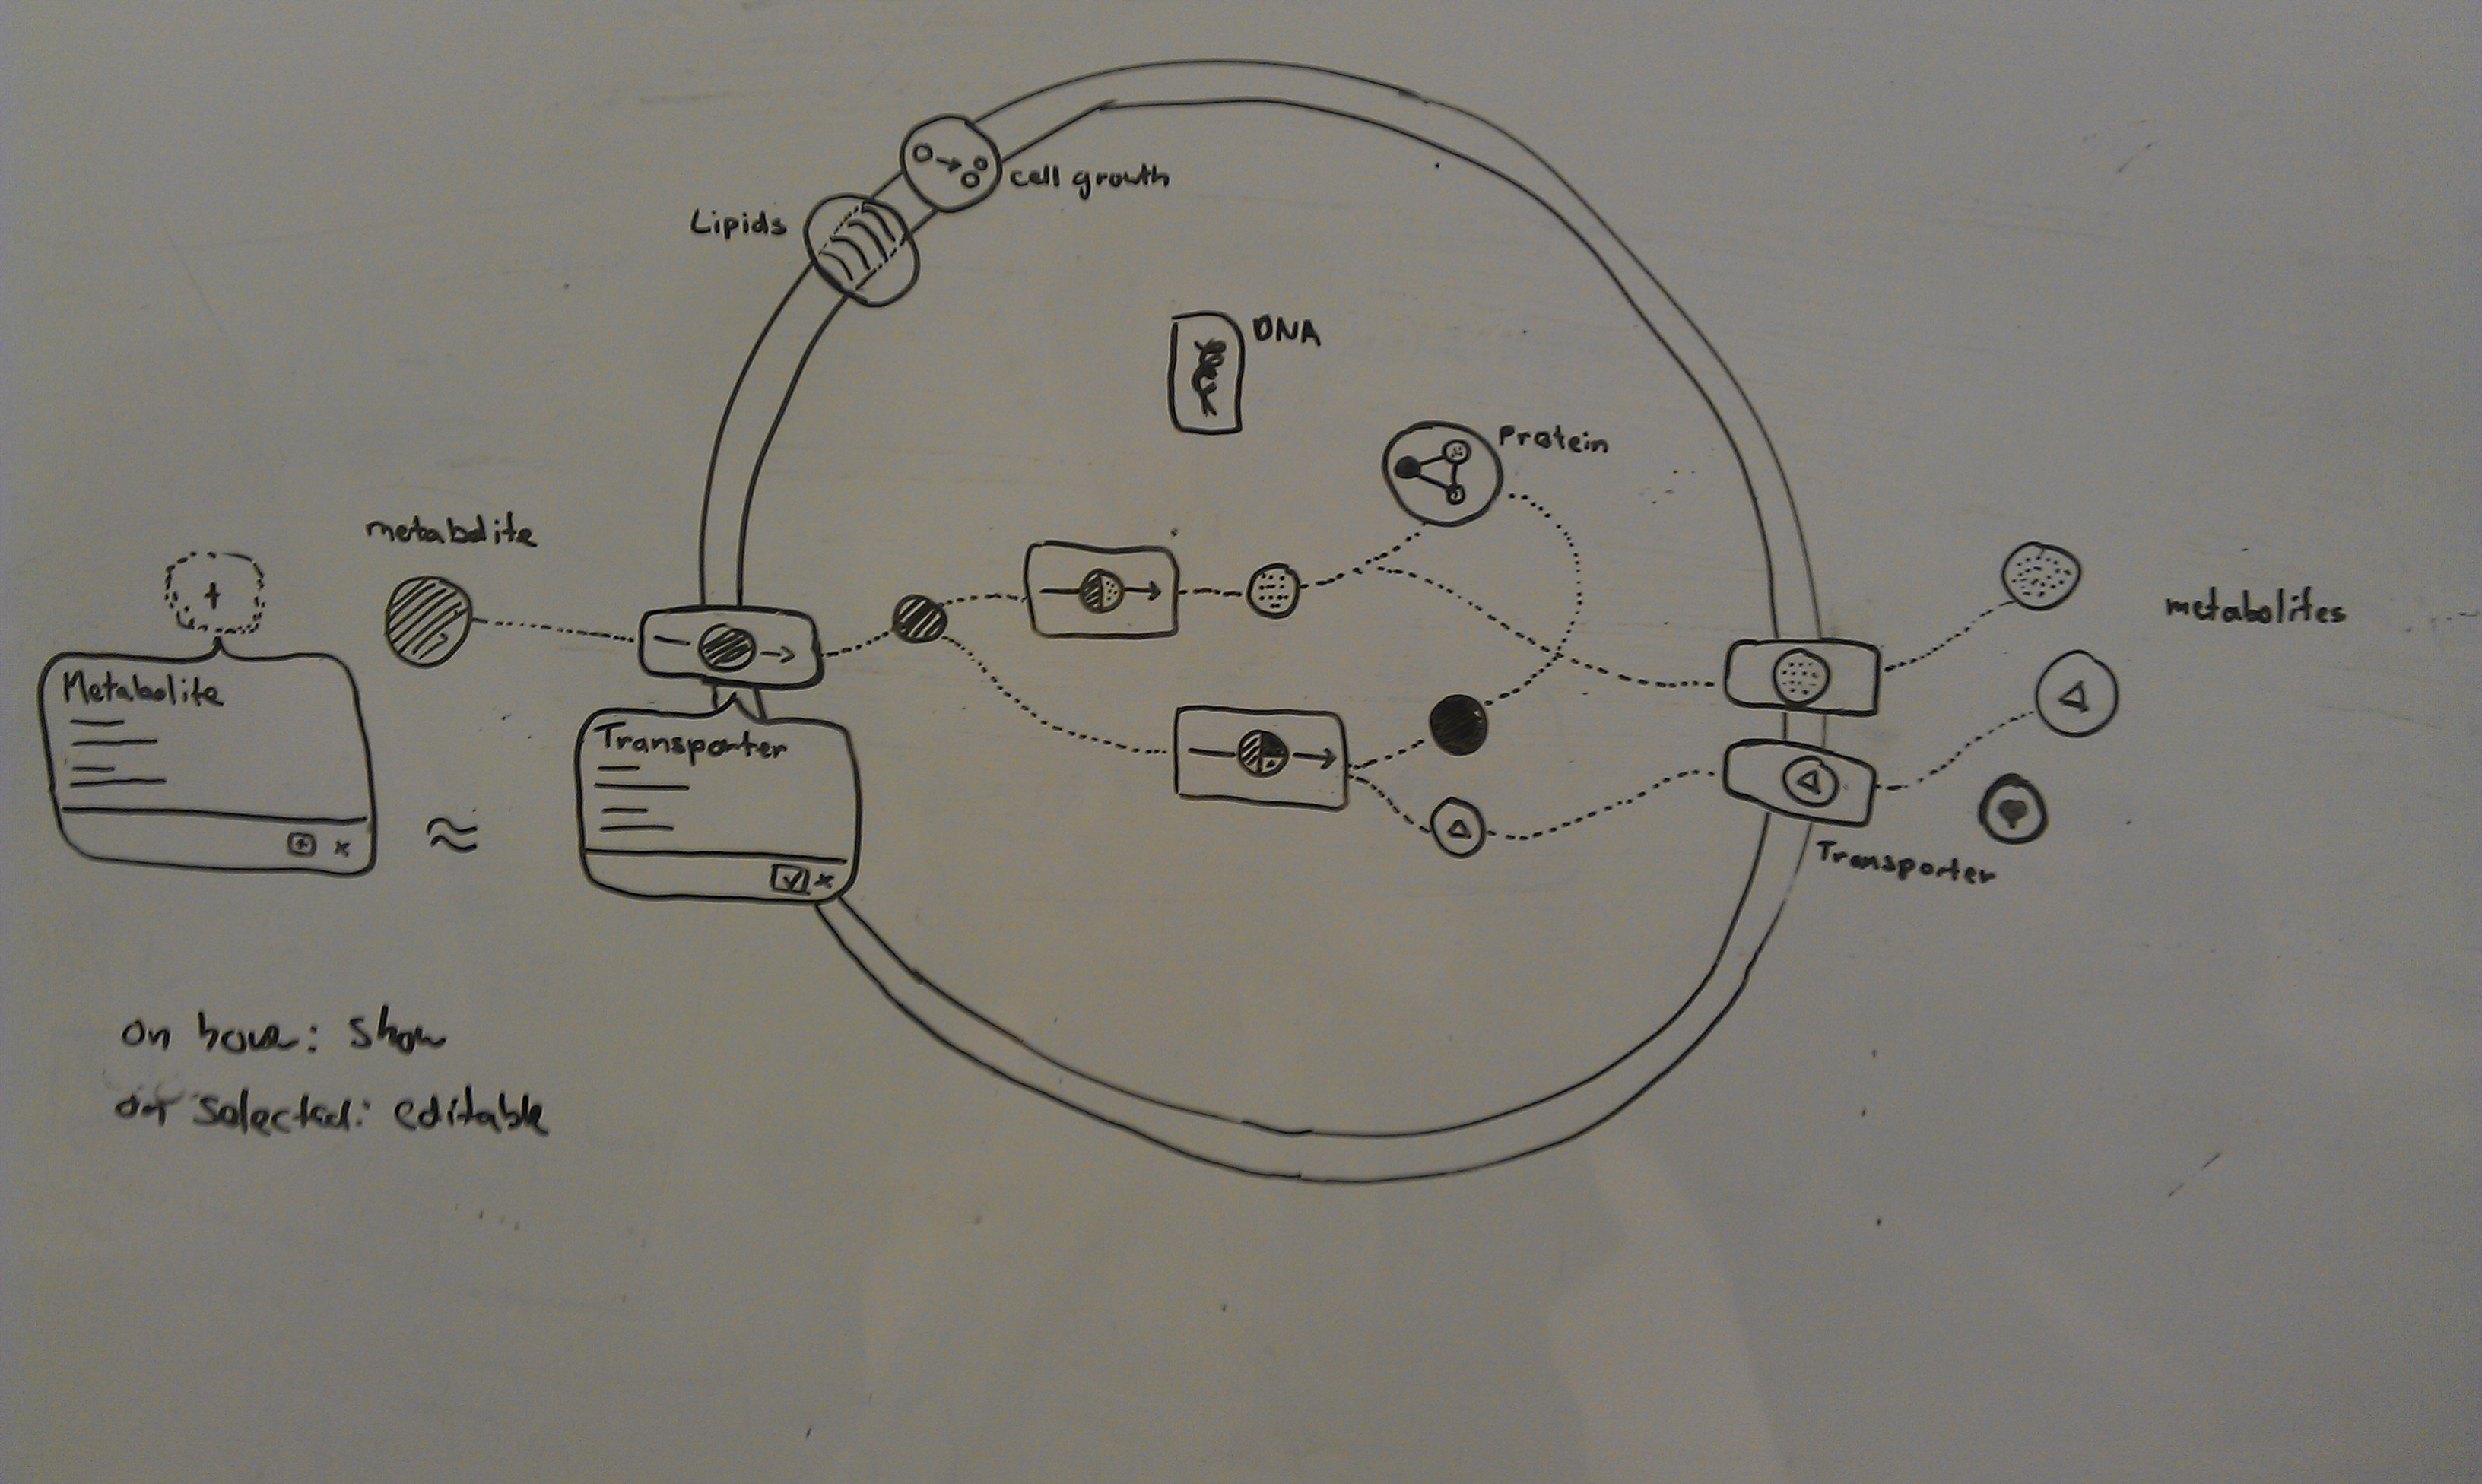
\includegraphics[scale=0.15]{mockup.jpg}}
			\caption{Mockup}
			\label{fig: Mockup}
		\end{figure}	
	\section{Product backlog}
		The product backlog is a list of possible features that gives a high-level description of the functionality that needs to be implemented before the application actually contains the feature. The priority of each story is defined by its position in the backlog. The higher on the backlog, the more important the item is and the more descriptive its required functionality is. Items that have been defined clearly enough also get a rough estimate of the amount of man-hours required to fully implement the feature described in that item.
		\\
		\textbf{A user can create a cell consisting of modules}. \\
		\indent
			\textit{Note: modules are processes like transporters bringing in substrates or ejecting products\\
		\indent
			Modules can be selected from a list and placed in the cell.\\
		\indent
			Estimate: 6 hours} \\
		\textbf{A user can see the output of the simulation. }\\
		\indent
			\textit{Note: a visual representation of the reactions with a module in the form of graphs. \\
		\indent
			Estimate: 4 hours} \\\
		\textbf{A user can change the module properties such as the reaction speed.} \\
		\indent
			\emph{Estimate: 8 hours} \\
		\textbf{A user can add substrates to the cell.} \\
		\indent
			\emph{Estimate: 4 hours} \\
		\textbf{A user can generate an HTML report of the simulation. This contains parameter values and concentration graphs from all the modules.} \\
		\indent
			\emph{ Estimate: 12 hours} \\
		\textbf{A user can generate PDF and Excel reports, equivalent to the HTML report.} \\
		\indent
			\emph{Estimate: 4 hours} \\
		\textbf{A user can save and load a model.} \\
		\indent
			\emph{Estimate: 8 hours} \\
		\textbf{A user can navigate the history of the cell to be able to undo actions and resume from an arbitrary point in the history of the cell.}\\
		\indent
			\emph{Estimate: 12 hours}\\
		\textbf{A user gets feedback on his model, such as missing modules, errors, constraints and possible optimisations if possible (maximising the yield, for example).} \\
		\indent
			\emph{Estimate: 12 hours} \\
		\textbf{A user can import and export cells in SBML-format}\\
		\indent
			\emph{Estimate: 10 hours}\\
		\textbf{A user can change the equations representing the different reactions.} \\
		\indent
			\emph{Estimate: 4 hours} \\
		\textbf{A user can change the language.} \\
		\indent
			\emph{Estimate: 8 hours} \\
		\textbf{A user can select parameter sets for modules based on existing DNA sequences known to generate a module with such reaction parameters.} \\
		\textbf{A user can view a phenotype of a model on his/her phone.} \\
		\textbf{A user can edit a cell model on his phone.} \\
		\textbf{A user can create new modules on his phone.} \\
		\textbf{A user can add modules to an existing cell model.} \\

	\clearpage
	\section{Definition of done}
		Defining when the following are done is important to keep the project flow consistent and make sure the product is deliverable. \\
		\\
		\textbf{Task:} If all the items from the task description are completed and this can be verified with one or more \emph{user} and/or an \emph{integration} tests. This is important because features have to be complete, otherwise there will be unfinished code in the system causing instability.\\
		\newline
		\textbf{User Story:} If the story is fulfilled and this can be tested with one or more \emph{acceptance tests}. This is important because the user stories are the basis for defining the functions the system must provide.\\
		\newline
		\textbf{Sprint:} Sunday 23:59. This is important because it limits the amount of work done during a sprint, forcing a controlled workflow.\\
		\newline
		(version of a) \textbf{Product/Release:} If the product can be shipped to the \emph{stakeholder}. This is important because this is what the stakeholder gets to see. It can be shipped when all features which are considered a MUST and SHOULD are implemented, see the high-level product backlog and roadmap. \\
		\newline
		\textbf{Project:} Never or when the \emph{stakeholder} decides (\emph{June 14$^{th}$}).

	\section{Glossary}
		\textbf{Backlog Item}\\
		A unit of work small enough to be completed by a team in one sprint iteration. Backlog items are decomposed into one or more tasks. \\
		\\
		\textbf{Demo}\\
		A session of testing with one or more stakeholders, where they evaluate the product.\\
		\\
		\textbf{Release}\\
		The transition of an increment of potentially shippable product from the development team into routine use by customers. Releases typically happen when one or more sprints has resulted in the product having enough value to outweigh the cost to deploy it.\\
		\\
		\textbf{Sprint} \\
		A one week period during which the team selects features of a product from the product backlog and finishes it by the end of the week. \\
		\\
		\textbf{Task} \\
		A sprint task (or task) is a unit of work small enough to be completed by a team member in a matter of hours. \\
		\\
		\textbf{User Story} \\
		One or more sentences in the everyday or business language of the end user that capture which action a user should perform to accomplish a specific goal with the product. The basis for defining the functions a business system must provide.
\end{document}

